\documentclass[12pt]{article}


\usepackage{amsmath}
\usepackage{amssymb}
\usepackage{amsfonts}
\usepackage{psfrag}
\usepackage{listings}

\usepackage{latexsym}
\usepackage{graphicx}
\usepackage{colonequals}

%\setlength\topmargin{-1in}
%\setlength{\oddsidemargin}{-0.5in}
%\setlength{\evensidemargin}{1.0in}

%\setlength{\parskip}{3pt plus 2pt}
%\setlength{\parindent}{30pt}
%\setlength{\marginparsep}{0.75cm}
%\setlength{\marginparwidth}{2.5cm}
%\setlength{\marginparpush}{1.0cm}
%\setlength{\textwidth}{7.5in}
%\setlength{\textheight}{10in}


\usepackage{listings}

\newcommand{\pset}[1]{ \mathcal{P}(#1) }
\newcommand{\partset}[1]{ \mathcal{P}^{*}(#1) }
\newcommand{\st}[0]{ \textrm{ s.t. } }
\newcommand{\fall}[0] { \textrm{ for all } }
\newcommand{\wrt}[0] { \textrm{ w.r.t. } }
\newcommand{\aew}[0] { \textrm{a.e.} }

\newcommand{\nats}[0] { \mathbb{N}}
\newcommand{\reals}[0] { \mathbb{R}}
\newcommand{\cmplxs}[0] { \mathbb{C}}
\newcommand{\complexes}[0] { \mathbb{C}}
\newcommand{\exreals}[0] {  [-\infty,\infty] }
\newcommand{\eps}[0] {  \epsilon }
\newcommand{\A}[0] { \mathcal{A} }
\newcommand{\B}[0] { \mathcal{B} }
\newcommand{\C}[0] { \mathcal{C} }
\newcommand{\D}[0] { \mathcal{D} }
\newcommand{\E}[0] { \mathcal{E} }
\newcommand{\F}[0] { \mathcal{F} }
\newcommand{\G}[0] { \mathcal{G} }
\newcommand{\M}[0] { \mathcal{M} }
\newcommand{\cS}[0] { \mathcal{S} }

\newcommand{\om}[0] { \omega }
\newcommand{\Om}[0] { \Omega }

\newcommand{\Bl}[0] { \mathcal{B} \ell }
\newcommand{\Ell}[0] { \mathcal{L} }

\renewcommand{\Re}{ \operatorname{Re} }
\renewcommand{\Im}{ \operatorname{Im} }

\newcommand{\IF}[0] { \; \textrm{if} \; }
\newcommand{\THEN}[0] { \; \textrm{then} \; }
\newcommand{\ELSE}[0] { \; \textrm{else} \; }
\newcommand{\AND}[0]{ \; \textrm{ and } \;  }
\newcommand{\OR}[0]{ \; \textrm{ or } \; }

\newcommand{\rimply}[0] { \Rightarrow }
\newcommand{\limply}[0] { \Leftarrow }
\newcommand{\rlimply}[0] { \Leftrightarrow }
\newcommand{\lrimply}[0] { \Leftrightarrow }

\newcommand{\rarw}[0] { \rightarrow }
\newcommand{\larw}[0] { \leftarrow }

\newcommand{ \defeq }[0] { \colonequals }
\newcommand{ \eqdef }[0] { \equalscolon }
%\newcommand{ \cf }[1] { \chi_{_{#1}} }
\newcommand{ \cf }[1] { \mathbf{1}_{#1} }

\newtheorem{thm}{Theorem}[section]

\title{Girsanov change of measure applied to Boundary value problems}
\date{April 27, 2010}
\author{Bernard Bodmann, Nick Maxwell}



\begin{document}


\maketitle

\section*{Theory}

{\bf Theorem 1:} (Girsanov) Let $W(t) \in \reals^n$ be a Brownian motion with respect to the measure $P$,  and $X(t) \in \reals^n$ an It\^o process given by 

$$
dX(t) = a(t,\om) dt + dW(t), \; \; 0 \le t \le T \le \infty.
$$

\noindent
Where $a:[0,T] \times \Om \rarw \reals^n$ is the drift. Then with

$$
M(t, \om ) = \exp \left( - \int_0^t a(s,\om) \cdot dW(s) - \frac{1}{2} \int_0^t a^2(s,\om) \, ds  \right), \; \; 0 \le t \le T
$$

\noindent
define the measure $Q$ by 

$$
dQ(\om) = M(T, \om) dP(\om),
$$

\noindent
then $X(t)$ is an $N$-dimensional Brownian motion wirh respect to $Q$. \\



{\bf Theorem 2:} Let $D \subset \reals^n$, open and connected, $\partial D$ its boundary, and $f: \partial D \rarw \reals$. Let $W(t)$, $X(t)$, $M(t)$, as in the last theorem. Define

$$
\tau_{x}(\om) = \inf \left( \left\{  0 \le t \le T;  X(t, \om) \not \in D,  \right\} \right),
$$

\noindent
where $X(0) = x$. Then

$$
u(x) = \int_\Om f ( X(\tau_x(\om), \om) ) \, M(\tau_x(\om), \om) \,  dP(\om) = E_{Q_x} [ f(X(\tau_x)) ],
$$

\noindent
where $dQ_x(\om) = M(\tau_x(\om), \om) dP(\om)$, solves the equation 

$$
\nabla^2 u(x) = \left \{ \begin{array}{cc} 
0, & x \in D \\
f(x), & x \in \partial D. \\
\end{array} \right.
$$\\

{\bf Idea:}
The drift, $a(t,\om)$, may be chosen to increase the rate of convergence in the above integral.

%\addvspace{5pt} \hrule

\section*{Experiment}

{\bf Verifying the hitting distribution in $\reals^2$:}  \\

Let $D$ be the open disc $\{x \in \reals^2; ||x||_2 < 1 \}$, so that $\partial D = \{ x \in \reals^2; ||x||_2 = 1 \}$, and take $f: \partial D \rarw (-\pi,\pi]$, such that $x = (\cos(f(x)), \sin(f(x)))$ for all $x \in \partial D$, i.e. $f$ is the function atan2 (see Wikipedia). Then let $Y_{x_0} = f(X(\tau_{x_0}))$, which is the hitting position of $X$, where $X(0) = {x_0} \in D$; we'll examine the distributions $E \mapsto P(Y_{x_0}^{-1}(E))$, and $E \mapsto Q(Y_{x_0}^{-1}(E))$ for measurable sets $E \subset (-\pi,\pi]$. $Y_{x_0}^{-1}(E) = \{ f(X(\tau_{x_0})) \in E_k\}$.\\

If $a \equiv 0$, then $X(t) = W(t)$, the standard Brownian motion, and in this case $P = Q$. So, for a given $x_0$, we expect that the distribution $E \mapsto P(Y_{x_0}^{-1}(E))$ with $a \equiv 0$ equals the distribution $E \mapsto Q(Y_{x_0}^{-1}(E))$ for an arbitrary $a$, which is the design of the measure $Q$. This is what we verify. \\

To sample $X(\tau_{x_0})$, the random hitting position, we discretize time into even steps of length $dt$, then take each $dW(t)=\sqrt{dt} N(0,1)$, where $N(0,1)$ is a vector of normally distributed random varaibles, with 0 mean and standard deviation 1. $X$ is started as $X=x_0$, and incremented as $X(t+dt) = dW(t) + a(t)dt$. Similarly, $\log(M)$ computed as the sum of $-a(t) \cdot dW(t) - \frac{1}{2} a(t) \cdot a(t) dt$. This process is continued until $X$ no longer is in the region $D$; in this case, untill $||X(t)||_2 > 1$. The final value of $X(t)$ is then $X(\tau_{x_0})$, and the final value of the sum of $\log(M(t))$ is then exponentiated to give $M(\tau_{x_0})$. \\

We partition the interval $(-\pi,\pi]$ into a number of disjoint, evenly spaced sub intervals, $\{ E_k \}$. For each sample $f(X(\tau_{x_0}))$, we check in which of the invervals, $\{ E_k \}$, it falls in. Two sums are associated to each $E_k$, and given that $f(X(\tau_{x_0}))$ fell in $E_k$, the first associated sum is incremented by $M(\tau_{x_0})$, and the second by 1. Finally, each sum is divided by the total number of samples, so that for each $E_k$, the first sum approximates $Q(Y_{x_0}^{-1}(E_k) = Q(\{ f(X(\tau_{x_0})) \in E_k\})$, and the second sum approximates $P(Y_{x_0}^{-1}(E_k)) = P(\{ f(X(\tau_{x_0})) \in E_k\})$, which are the desired ditributions. \\


\begin{figure}[h]
\begin{center}
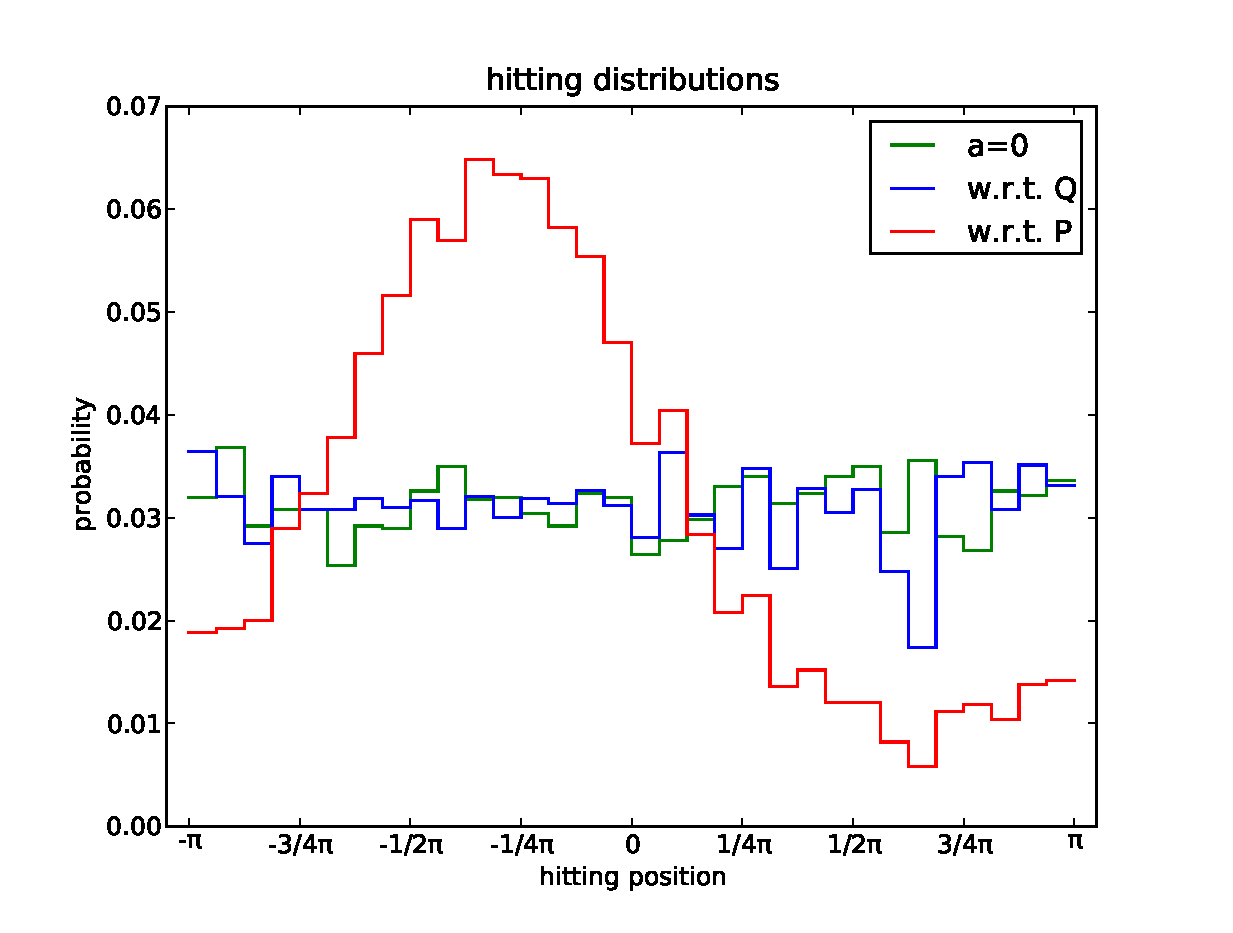
\includegraphics[width=5in]{figure1.eps}
\end{center}
\caption{Results, with $a(t) = (-0.7, 0.5 )$, $x_0 = (0.0, 0.0)$, $dt=0.02$, 32 partitions of $(-\pi,\pi]$, and 5000 samples.}
\end{figure}


\begin{figure}[h]
\begin{center}
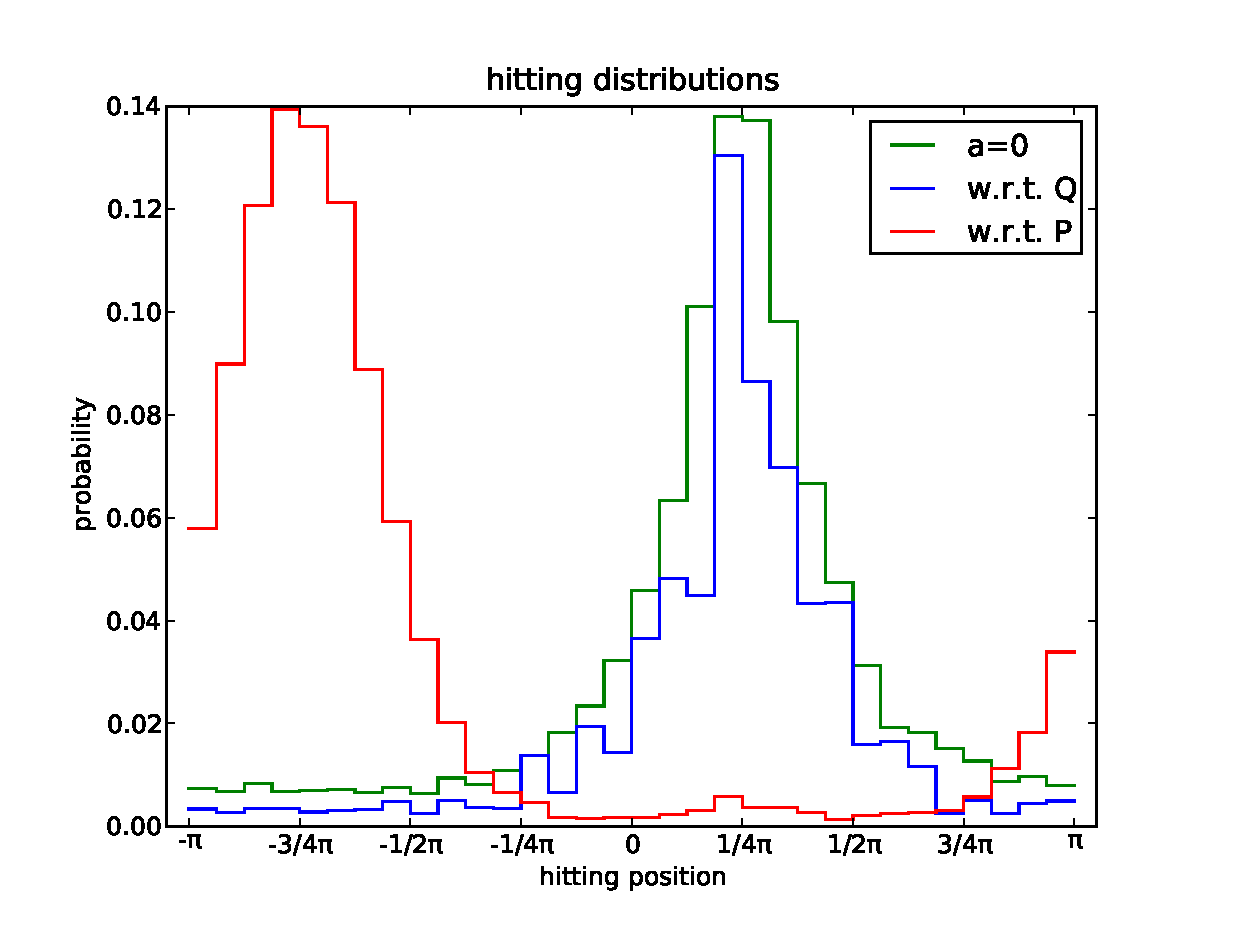
\includegraphics[width=5in]{figure2.eps}
\end{center}
\caption{Results, with $a(t) = (-4.0,-4.0) + \xi (t+1)^2$, where $\xi$ is a uniformly distributed random variable on $[-\frac{1}{2},\frac{1}{2}]$ , $x_0 = (0.5, 0.5)$, $dt=0.02$, 32 partitions of $(-\pi,\pi]$, and 10,000 samples.}
\end{figure}


{\bf Verifying the hitting distribution in $\reals^n$:}  \\

Let $D$ be the open sphere $\{x \in \reals^n; ||x||_2 < 1 \}$, so that $\partial D = \{ x \in \reals^n; ||x||_2 = 1 \}$. Then we define an enumeration of the quadrants of $\reals^n$  as folows. For some $x = (x_1, x_2, ..., x_n) \in \reals^n$, if $x_k \ge 0$, let $s_k=2^k$, otherwise let $s_k=0$, then take $f(x) = \sum_{k=0}^{n-1} s_k$. Then we'll follow the same steps as in the $\reals^2$ case, now with $E_k = \{ k \}$, for $0 \le k < 2^n$. \\


\begin{figure}[h]
\begin{center}
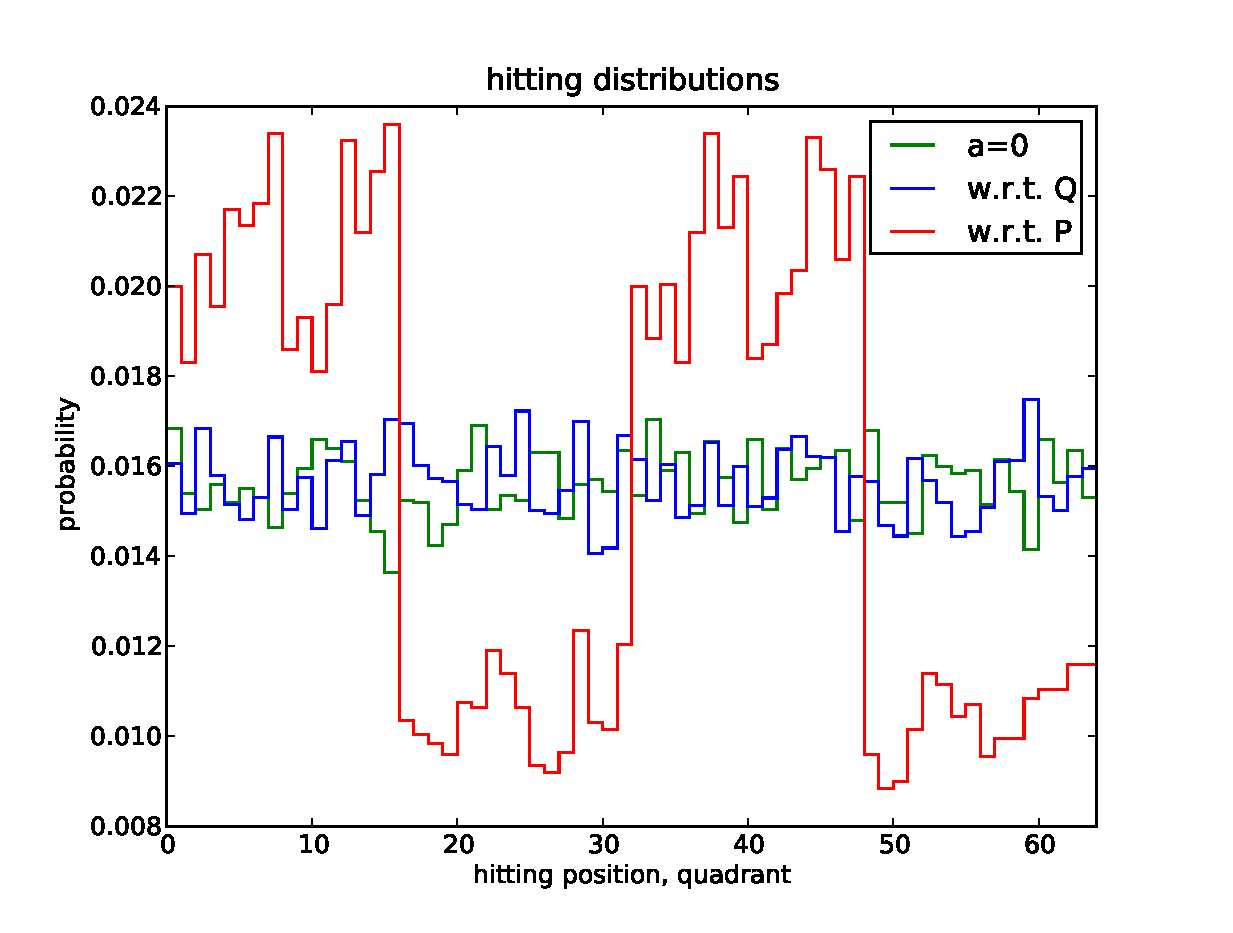
\includegraphics[width=5in]{figure5.eps}
\end{center}
\caption{Results, in 6 dimensions, with $a(t) = (0,0,0.2,0,-0.9,0)$, $x_0 = 0$, $dt=0.03$, and 20,000 samples.}
\end{figure}







\break




\end{document}


